% --------------------------------------------------------------
% This is all preamble stuff that you don't have to worry about.
% Head down to where it says "Start here"
% --------------------------------------------------------------

\documentclass[12pt]{article}

\usepackage[margin=1in]{geometry}
\usepackage{amsmath,amsthm,amssymb}
\usepackage{tikz}

\newcommand{\N}{\mathbb{N}}
\newcommand{\Z}{\mathbb{Z}}

\newenvironment{theorem}[2][Theorem]{\begin{trivlist}
\item[\hskip \labelsep {\bfseries #1}\hskip \labelsep {\bfseries #2.}]}{\end{trivlist}}
\newenvironment{lemma}[2][Lemma]{\begin{trivlist}
\item[\hskip \labelsep {\bfseries #1}\hskip \labelsep {\bfseries #2.}]}{\end{trivlist}}
\newenvironment{exercise}[2][Exercise]{\begin{trivlist}
\item[\hskip \labelsep {\bfseries #1}\hskip \labelsep {\bfseries #2.}]}{\end{trivlist}}
\newenvironment{question}[2][Question]{\begin{trivlist}
\item[\hskip \labelsep {\bfseries #1}\hskip \labelsep {\bfseries #2.}]}{\end{trivlist}}
\newenvironment{proposition}[2][Proposition]{\begin{trivlist}
\item[\hskip \labelsep {\bfseries #1}\hskip \labelsep {\bfseries #2.}]}{\end{trivlist}}
\newenvironment{corollary}[2][Corollary]{\begin{trivlist}
\item[\hskip \labelsep {\bfseries #1}\hskip \labelsep {\bfseries #2.}]}{\end{trivlist}}

\begin{document}

% --------------------------------------------------------------
%                         Start here
% --------------------------------------------------------------

%\renewcommand{\qedsymbol}{\filledbox}

\title{Homework 3}%replace X with the appropriate number
\author{Dustin Lambright - dalambri \\ Aseem Raina - araina \\ Bihan Zhang - bzhang28\\ %replace with your name
CSC 565 - Graph Theory} %if necessary, replace with your course title

\maketitle


\begin{question}{1}
Show that every simple graph $G$ with 6 vertices has either a clique of size 3 or an independent
set of size 3.
\end{question}

By the definition of inependent sets and cliques, any graph G with a clique of size n will also have a clique of n-1, n-2, ... n-(n-1).  The same goes for an independent set.  Therefore, using contradiction, if a graph does not have a clique of size 3 and does not have an independent set of size 3, the statement is false. \\ \\

The graph $K_{1,5}$ has a maximum clique size of 2, but an independent set of 5. (displayed in red)
\begin{align*}
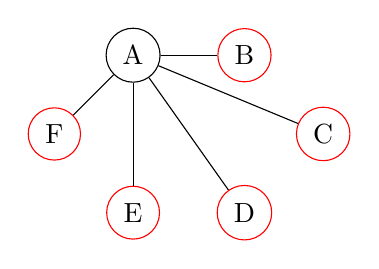
\begin{tikzpicture}
\node[shape=circle,draw=black] (A) at (1,2) {A};
\node[shape=circle,draw=red] (B) at (2.4142857,2) {B};
\node[shape=circle,draw=red] (C) at (3.4142856,1) {C};
\node[shape=circle,draw=red] (D) at (2.4142857,0) {D};
\node[shape=circle,draw=red] (E) at (1,0) {E};
\node[shape=circle,draw=red] (F) at (0,1) {F};
\path [] (A) edge node[left] {} (B);
\path [] (A) edge node[left] {} (C);
\path [] (A) edge node[left] {} (D);
\path [] (A) edge node[left] {} (E);
\path [] (A) edge node[left] {} (F);
\end{tikzpicture}
\end{align*}

In an effort to reduce the size of the maximum independent set, edges are replaced, creating a cyclic graph: \\

\begin{align*}
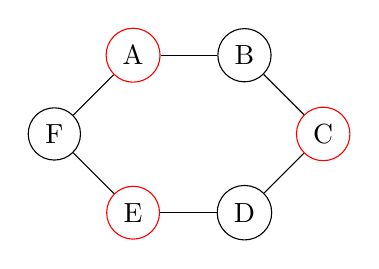
\begin{tikzpicture}
\node[shape=circle,draw=red] (A) at (1,2) {A};
\node[shape=circle,draw=black] (B) at (2.4142857,2) {B};
\node[shape=circle,draw=red] (C) at (3.4142856,1) {C};
\node[shape=circle,draw=black] (D) at (2.4142857,0) {D};
\node[shape=circle,draw=red] (E) at (1,0) {E};
\node[shape=circle,draw=black] (F) at (0,1) {F};
\path [] (A) edge node[left] {} (B);
\path [] (B) edge node[left] {} (C);
\path [] (C) edge node[left] {} (D);
\path [] (D) edge node[left] {} (E);
\path [] (F) edge node[left] {} (A);
\path [] (E) edge node[left] {} (F);
\end{tikzpicture}
\end{align*}

This graph has a a maximum independent set of 3, and a maximum clique of 2. The only way to reduce the size of an independent set, i.e., $\{A,E,C\}$ is to connect any of those vertices with an edge.  The connection of any of these vertices results in a clique of size 3.  In an effort to maintain our clique constraint, if we remove the edges AF and AB to connect the independent set $\{A,E,C\}$, we end up with an independent set $\{A,F,B, D\}$.

\begin{align*}
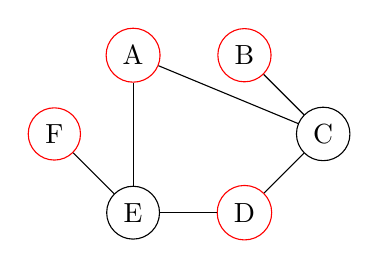
\begin{tikzpicture}
\node[shape=circle,draw=red] (A) at (1,2) {A};
\node[shape=circle,draw=red] (B) at (2.4142857,2) {B};
\node[shape=circle,draw=black] (C) at (3.4142856,1) {C};
\node[shape=circle,draw=red] (D) at (2.4142857,0) {D};
\node[shape=circle,draw=black] (E) at (1,0) {E};
\node[shape=circle,draw=red] (F) at (0,1) {F};
\path [] (A) edge node[left] {} (C);
\path [] (B) edge node[left] {} (C);
\path [] (C) edge node[left] {} (D);
\path [] (D) edge node[left] {} (E);
\path [] (E) edge node[left] {} (A);
\path [] (E) edge node[left] {} (F);
\end{tikzpicture}
\end{align*}

The graph $C_6$ is the closest we can get to a graph without a clique of size 3 and without an independent set of size 3, but it has an independent set of size three, proving that a graph with a vertex count of 6 has to have an independent set of size 3 or a clique of size 3.

\begin{question}{2}
Prove or disprove: In a simple graph, every closed even trail of length more than 3 contains an
even cycle.
\end{question}

\begin{question}{3}
Prove the following by strong induction on the length of the trail: The edge set of every closed
trail can be partitioned into zero or more pairwise edge-disjoint cycles.
\end{question}

\begin{question}{4}
Suppose that T is a maximal trail in a simple graph G and that T has at least one edge and is
not closed. Prove that the endpoints of T have odd degree.
\end{question}

\begin{question}{5}
If $G$ is a graph with vertices $v_1, v_2, . . . , v_n$ and $A^k$ denotes the kth power of the adjacency matrix
of $G$ under matrix multiplication then \\ \\

(***) $A^{k}[i, j]$ is the number of $v_i, v_j$ -walks of length $k$ in $G$. \\ \\

Show how to use (***) to solve the following without multipltying matrices and prove your answer
correct: Let A be the adjacency matrix of $K_n$. If $i = j$, then $A^3[i, j]$ =\_\_\_\_ . Otherwise
$A^{3}[i, j]$ = \_\_\_\_.
\end{question}

Consider the graph $K_3$, whose vertex count is $n$.
\begin{align*}
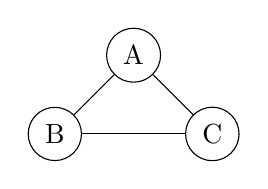
\begin{tikzpicture}
\node[shape=circle,draw=black] (A) at (1,1) {A};
\node[shape=circle,draw=black] (B) at (0,0) {B};
\node[shape=circle,draw=black] (C) at (2,0) {C};
\path [] (A) edge node[left] {} (B);
\path [] (A) edge node[left] {} (C);
\path [] (B) edge node[left] {} (C);
\end{tikzpicture}
\end{align*}

These two branches can be calculated as follows: 
\begin{center}
\Large TO CALCULATE (***) FOR $i \neq j$
\end{center}
\normalsize

There are 3 possible paths from A to C. \\
\begin{center}
\begin{tabular}{|c|}  \hline
\{AC, CA, AC\} \\
\{AC, CB, BC\} \\
\{AB, BA, AC\} \\ \hline
\end{tabular}
\end{center}

To calculate the number of walks from A to C, we need to break down the number of moves needed from two branches: going to C, and not going to C
\begin{center}
\begin{tabular}{|c|}  \hline
\{AC, CA, AC\} \\
\{AC, CB, BC\} \\ \hline
\{AB, BA, AC\} \\ \hline
\end{tabular}


\begin{tabular}{|c|c|c|}
\multicolumn{3}{c}{BEGINNING MOVE TO C (THE END POINT)}  \\ \hline
MOVE TO & OPTIONS & REASONING \\ \hline
C & 1 & You can only move to C, as per definition \\ \hline
A or B &$n-1$ & Any option but C works for this step \\ \hline
C & 1 & The walk's third step has to end on C \\ \hline
\end{tabular} \\


\begin{tabular}{|c|c|c|}
\multicolumn{3}{c}{BEGINNING MOVE TO ANY POINT (THE END POINT)}  \\ \hline
MOVE TO & OPTIONS & REASONING \\ \hline
B & $n-2$ & You can only move to any vertex that isn't C \\ \hline
A or C & $n-2$ & C cannot be the choice in this step \\ \hline
C & 1 & The walk's third step has to end on C \\ \hline
\end{tabular} \\
\end{center}

If we add these two options together, we get $(1 \times (n-1) \times 1) +  ((n-2) \times (n-2) \times 1)$, which simplifies to $n^{2} - 3n +3$. \\


The formula for calculating (***) $A^{3}[i, j]$ where $i \neq j$ therefore is $n^{2} -3n + 3$.

\begin{center}
\Large TO CALCULATE (***) FOR $i = j$
\end{center}
\normalsize

There are 2 possible paths from A to A. \\
\begin{center}
\begin{tabular}{|c|}  \hline
\{AB, BC, CA\} \\
\{AC, CB, BA\} \\ \hline
\end{tabular}
\end{center}

To calculate the number of paths, we have the following options: \\
\begin{center}
\begin{tabular}{|c|c|c|}
\multicolumn{3}{c}{STARTING AND ENDING AT THE SAME POINT}  \\ \hline
MOVE TO & OPTIONS & REASONING \\ \hline
B or A & $n-1$ & Any option will work on this step \\ \hline
A or B &$n-2$ & Any option will work, except for C \\ \hline
C & 1 & The walk's third step has to end on C \\ \hline
\end{tabular} \\
\end{center}

When we combine these, we get $(n-1) \times (n-2) \times 1$, which simplifies to $n^{2} -3n + 2$.

The formula for calculating (***) $A^{3}[i, j]$ where $i = j$ therefore is $n^{2} -3n + 2$.

\begin{center}
\Large IN CONCLUSION \\

\normalsize
$ A^{3}[i,j] = $ 
    $\begin{cases} n^{2} -3n + 3  & \mbox{if } i \neq  j  \\  n^{2} -3n + 2   & \mbox{if } i =j \\   \end{cases}$ \\
    where $n$ is the number of vertices in $G$.
\end{center}

\begin{question}{6}
Draw a simple, connected graph with the following degree sequence, or prove that no such graph
is possible: \\
a. (3, 3, 3, 2, 2, 2) \\
b. (7, 6, 5, 4, 3, 2, 1) \\ 
c. (3, 3, 2, 2, 1, 1) \\
d. (7, 6, 5, 4, 3, 3, 2) \\
e. (6, 6, 5, 4, 3, 3, 1) 
\end{question}

\begin{question}{7}
 How many different simple graphs are there with 5 edges and with vertex set {v1, v2, . . . v5}?
(We are counting labeled graphs, not isomorphism classes)
\end{question}

\begin{question}{8}
Prove by contradiction: A graph with every vertex degree even has no cut-edge.
\end{question}




% --------------------------------------------------------------
%     You don't have to mess with anything below this line.
% --------------------------------------------------------------

\end{document}
